
    \item A horizontal circular platform of radius 0.5 m and mass 0.45 kg is free to rotate about its axis. Two massless spring toy-guns, each carrying a steel ball of mass 0.05 kg are attached to the platform at a distance 0.25 m from the centre on its either sides along its diameter (see figure). Each gun simultaneously fires the balls horizontally and perpendicular to the diameter in opposite directions. After leaving the platform, the balls have horizontal speed of 9 m\textsuperscript{-1} with respect to the ground. The rotational speed of the platform in\textsuperscript{-1} after the balls leave the platform is \underline{\hspace{2.5 cm}}.

    \begin{center}
        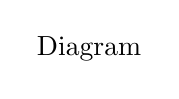
\begin{tikzpicture}
            \node {Diagram};
        \end{tikzpicture}
    \end{center}
